% Options for packages loaded elsewhere
\PassOptionsToPackage{unicode}{hyperref}
\PassOptionsToPackage{hyphens}{url}
%
\documentclass[
]{book}
\usepackage{amsmath,amssymb}
\usepackage{iftex}
\ifPDFTeX
  \usepackage[T1]{fontenc}
  \usepackage[utf8]{inputenc}
  \usepackage{textcomp} % provide euro and other symbols
\else % if luatex or xetex
  \usepackage{unicode-math} % this also loads fontspec
  \defaultfontfeatures{Scale=MatchLowercase}
  \defaultfontfeatures[\rmfamily]{Ligatures=TeX,Scale=1}
\fi
\usepackage{lmodern}
\ifPDFTeX\else
  % xetex/luatex font selection
\fi
% Use upquote if available, for straight quotes in verbatim environments
\IfFileExists{upquote.sty}{\usepackage{upquote}}{}
\IfFileExists{microtype.sty}{% use microtype if available
  \usepackage[]{microtype}
  \UseMicrotypeSet[protrusion]{basicmath} % disable protrusion for tt fonts
}{}
\makeatletter
\@ifundefined{KOMAClassName}{% if non-KOMA class
  \IfFileExists{parskip.sty}{%
    \usepackage{parskip}
  }{% else
    \setlength{\parindent}{0pt}
    \setlength{\parskip}{6pt plus 2pt minus 1pt}}
}{% if KOMA class
  \KOMAoptions{parskip=half}}
\makeatother
\usepackage{xcolor}
\usepackage{color}
\usepackage{fancyvrb}
\newcommand{\VerbBar}{|}
\newcommand{\VERB}{\Verb[commandchars=\\\{\}]}
\DefineVerbatimEnvironment{Highlighting}{Verbatim}{commandchars=\\\{\}}
% Add ',fontsize=\small' for more characters per line
\usepackage{framed}
\definecolor{shadecolor}{RGB}{248,248,248}
\newenvironment{Shaded}{\begin{snugshade}}{\end{snugshade}}
\newcommand{\AlertTok}[1]{\textcolor[rgb]{0.94,0.16,0.16}{#1}}
\newcommand{\AnnotationTok}[1]{\textcolor[rgb]{0.56,0.35,0.01}{\textbf{\textit{#1}}}}
\newcommand{\AttributeTok}[1]{\textcolor[rgb]{0.13,0.29,0.53}{#1}}
\newcommand{\BaseNTok}[1]{\textcolor[rgb]{0.00,0.00,0.81}{#1}}
\newcommand{\BuiltInTok}[1]{#1}
\newcommand{\CharTok}[1]{\textcolor[rgb]{0.31,0.60,0.02}{#1}}
\newcommand{\CommentTok}[1]{\textcolor[rgb]{0.56,0.35,0.01}{\textit{#1}}}
\newcommand{\CommentVarTok}[1]{\textcolor[rgb]{0.56,0.35,0.01}{\textbf{\textit{#1}}}}
\newcommand{\ConstantTok}[1]{\textcolor[rgb]{0.56,0.35,0.01}{#1}}
\newcommand{\ControlFlowTok}[1]{\textcolor[rgb]{0.13,0.29,0.53}{\textbf{#1}}}
\newcommand{\DataTypeTok}[1]{\textcolor[rgb]{0.13,0.29,0.53}{#1}}
\newcommand{\DecValTok}[1]{\textcolor[rgb]{0.00,0.00,0.81}{#1}}
\newcommand{\DocumentationTok}[1]{\textcolor[rgb]{0.56,0.35,0.01}{\textbf{\textit{#1}}}}
\newcommand{\ErrorTok}[1]{\textcolor[rgb]{0.64,0.00,0.00}{\textbf{#1}}}
\newcommand{\ExtensionTok}[1]{#1}
\newcommand{\FloatTok}[1]{\textcolor[rgb]{0.00,0.00,0.81}{#1}}
\newcommand{\FunctionTok}[1]{\textcolor[rgb]{0.13,0.29,0.53}{\textbf{#1}}}
\newcommand{\ImportTok}[1]{#1}
\newcommand{\InformationTok}[1]{\textcolor[rgb]{0.56,0.35,0.01}{\textbf{\textit{#1}}}}
\newcommand{\KeywordTok}[1]{\textcolor[rgb]{0.13,0.29,0.53}{\textbf{#1}}}
\newcommand{\NormalTok}[1]{#1}
\newcommand{\OperatorTok}[1]{\textcolor[rgb]{0.81,0.36,0.00}{\textbf{#1}}}
\newcommand{\OtherTok}[1]{\textcolor[rgb]{0.56,0.35,0.01}{#1}}
\newcommand{\PreprocessorTok}[1]{\textcolor[rgb]{0.56,0.35,0.01}{\textit{#1}}}
\newcommand{\RegionMarkerTok}[1]{#1}
\newcommand{\SpecialCharTok}[1]{\textcolor[rgb]{0.81,0.36,0.00}{\textbf{#1}}}
\newcommand{\SpecialStringTok}[1]{\textcolor[rgb]{0.31,0.60,0.02}{#1}}
\newcommand{\StringTok}[1]{\textcolor[rgb]{0.31,0.60,0.02}{#1}}
\newcommand{\VariableTok}[1]{\textcolor[rgb]{0.00,0.00,0.00}{#1}}
\newcommand{\VerbatimStringTok}[1]{\textcolor[rgb]{0.31,0.60,0.02}{#1}}
\newcommand{\WarningTok}[1]{\textcolor[rgb]{0.56,0.35,0.01}{\textbf{\textit{#1}}}}
\usepackage{longtable,booktabs,array}
\usepackage{calc} % for calculating minipage widths
% Correct order of tables after \paragraph or \subparagraph
\usepackage{etoolbox}
\makeatletter
\patchcmd\longtable{\par}{\if@noskipsec\mbox{}\fi\par}{}{}
\makeatother
% Allow footnotes in longtable head/foot
\IfFileExists{footnotehyper.sty}{\usepackage{footnotehyper}}{\usepackage{footnote}}
\makesavenoteenv{longtable}
\usepackage{graphicx}
\makeatletter
\def\maxwidth{\ifdim\Gin@nat@width>\linewidth\linewidth\else\Gin@nat@width\fi}
\def\maxheight{\ifdim\Gin@nat@height>\textheight\textheight\else\Gin@nat@height\fi}
\makeatother
% Scale images if necessary, so that they will not overflow the page
% margins by default, and it is still possible to overwrite the defaults
% using explicit options in \includegraphics[width, height, ...]{}
\setkeys{Gin}{width=\maxwidth,height=\maxheight,keepaspectratio}
% Set default figure placement to htbp
\makeatletter
\def\fps@figure{htbp}
\makeatother
\setlength{\emergencystretch}{3em} % prevent overfull lines
\providecommand{\tightlist}{%
  \setlength{\itemsep}{0pt}\setlength{\parskip}{0pt}}
\setcounter{secnumdepth}{5}
% Packages
\usepackage{booktabs}
\usepackage{xcolor}
\usepackage{floatrow}
%\usepackage[T1]{fontenc}
\usepackage{lmodern}

% Highlights
%% Definitions
\newcommand{\defi}[1]{\colorbox{yellow}{#1}}
%% Key words
\newcommand{\key}[1]{\colorbox{green}{#1}}
%% Formulas
\newcommand{\eq}[1]{\colorbox{orange}{#1}}
%% Names
\newcommand{\nam}[1]{\colorbox{pink}{#1}}
%% Proofs
\newcommand{\proofs}[1]{\colorbox{blue}{#1}}

% Set titles at the begining of the figure 
\floatsetup[figure]{capposition=top}

\ifLuaTeX
  \usepackage{selnolig}  % disable illegal ligatures
\fi
\usepackage[]{natbib}
\bibliographystyle{plainnat}
\usepackage{bookmark}
\IfFileExists{xurl.sty}{\usepackage{xurl}}{} % add URL line breaks if available
\urlstyle{same}
\hypersetup{
  pdftitle={Econometrics},
  pdfauthor={Mimi},
  hidelinks,
  pdfcreator={LaTeX via pandoc}}

\title{Econometrics}
\author{Mimi}
\date{2024-10-07}

\usepackage{amsthm}
\newtheorem{theorem}{Theorem}[chapter]
\newtheorem{lemma}{Lemma}[chapter]
\newtheorem{corollary}{Corollary}[chapter]
\newtheorem{proposition}{Proposition}[chapter]
\newtheorem{conjecture}{Conjecture}[chapter]
\theoremstyle{definition}
\newtheorem{definition}{Definition}[chapter]
\theoremstyle{definition}
\newtheorem{example}{Example}[chapter]
\theoremstyle{definition}
\newtheorem{exercise}{Exercise}[chapter]
\theoremstyle{definition}
\newtheorem{hypothesis}{Hypothesis}[chapter]
\theoremstyle{remark}
\newtheorem*{remark}{Remark}
\newtheorem*{solution}{Solution}
\begin{document}
\maketitle

{
\setcounter{tocdepth}{1}
\tableofcontents
}
\chapter*{About}\label{about}
\addcontentsline{toc}{chapter}{About}

This is a \emph{sample} book written in \textbf{Markdown}. You can use anything that Pandoc's Markdown supports; for example, a math equation \(a^2 + b^2 = c^2\).

\section{Usage}\label{usage}

Each \textbf{bookdown} chapter is an .Rmd file, and each .Rmd file can contain one (and only one) chapter. A chapter \emph{must} start with a first-level heading: \texttt{\#\ A\ good\ chapter}, and can contain one (and only one) first-level heading.

Use second-level and higher headings within chapters like: \texttt{\#\#\ A\ short\ section} or \texttt{\#\#\#\ An\ even\ shorter\ section}.

The \texttt{index.Rmd} file is required, and is also your first book chapter. It will be the homepage when you render the book.

\section{Render book}\label{render-book}

You can render the HTML version of this example book without changing anything:

\begin{enumerate}
\def\labelenumi{\arabic{enumi}.}
\item
  Find the \textbf{Build} pane in the RStudio IDE, and
\item
  Click on \textbf{Build Book}, then select your output format, or select ``All formats'' if you'd like to use multiple formats from the same book source files.
\end{enumerate}

Or build the book from the R console:

\begin{Shaded}
\begin{Highlighting}[]
\NormalTok{bookdown}\SpecialCharTok{::}\FunctionTok{render\_book}\NormalTok{()}
\end{Highlighting}
\end{Shaded}

To render this example to PDF as a \texttt{bookdown::pdf\_book}, you'll need to install XeLaTeX. You are recommended to install TinyTeX (which includes XeLaTeX): \url{https://yihui.org/tinytex/}.

\section{Preview book}\label{preview-book}

As you work, you may start a local server to live preview this HTML book. This preview will update as you edit the book when you save individual .Rmd files. You can start the server in a work session by using the RStudio add-in ``Preview book'', or from the R console:

\begin{Shaded}
\begin{Highlighting}[]
\NormalTok{bookdown}\SpecialCharTok{::}\FunctionTok{serve\_book}\NormalTok{()}
\end{Highlighting}
\end{Shaded}

\chapter{Econometrics}\label{intro}

\begin{itemize}
\item
  \defi{Econometrics}: Using statistical methods for estimating relationships in economics. It can be used to forecast and policy evaluation.

  \begin{itemize}
  \tightlist
  \item
    It uses \key{empirical data} to test assumptions, relationships and theories.
  \end{itemize}
\end{itemize}

\section*{How to start?}\label{how-to-start}
\addcontentsline{toc}{section}{How to start?}

\begin{itemize}
\item
  What is the question of interest?
\item
  An \key{economic model} may be needed to test economic theories; they are equations stating the relationship you are looking for. It determines the variables that should be included. Intuition can be also a starting point:

  \begin{itemize}
  \tightlist
  \item
    The relationship between wages and years of education: \(wages=f(y\_educ)\). It is expected that years of education increase wages.
  \end{itemize}
\item
  The \key{econometric model} specify the function of the economic model: Wages depend on the years of education and a term u.
\end{itemize}

\[wages=\beta_0+\beta_1y\_educ+u\]

\begin{itemize}
\item
  However, not every factor that affects wages can be observed or measured. The term \key{u} represent such unobserved factors, and the measuring error of the included variables. It can never be eliminated entirely. It is also called \key{error term} or \key{disturbance}
\item
  \(\beta_n\) are the \key{parameters}. They give information about the relationship between the independent and dependent variable.
\item
  After establishing the econometric model, we can start doing hypothesis about the parameters. Is the relationship positive, negative or zero?
\item
  Then, data is required to estimate the parameters of the established model. There are different types of data structures:
\end{itemize}

\subsection*{Cross-Sectional Data}\label{cross-sectional-data}
\addcontentsline{toc}{subsection}{Cross-Sectional Data}

\begin{itemize}
\item
  Sample of variety of units taken in a point in time. Minor timing differences in collecting the data are ignored.
\item
  The order of the observations doesn't matter.
\item
  \key{Random Sampling} is needed to get better results. It means the observations drawed are independent. However, it is not always appropriate to make this assumption.
\item
  \key{Random Sampling} is violated when population is not large enough, so the observations are not independent draws. It those cases, the same methodology has to be refined.
\item
  In some cases, \key{Random Sampling} can be checked if the descriptive statistics are \key{balanced}; for example, if we are making a comparison between women and men, the sample should be compound 50\% women and 50\% men, approximately.
\item
  An example of \key{cross-sectional data} using \textbf{dplyr} package \citep{dplyr} is shown below
\end{itemize}

\begin{verbatim}
## # A tibble: 87 x 14
##    name     height  mass hair_color skin_color eye_color birth_year sex   gender
##    <chr>     <int> <dbl> <chr>      <chr>      <chr>          <dbl> <chr> <chr> 
##  1 Luke Sk~    172    77 blond      fair       blue            19   male  mascu~
##  2 C-3PO       167    75 <NA>       gold       yellow         112   none  mascu~
##  3 R2-D2        96    32 <NA>       white, bl~ red             33   none  mascu~
##  4 Darth V~    202   136 none       white      yellow          41.9 male  mascu~
##  5 Leia Or~    150    49 brown      light      brown           19   fema~ femin~
##  6 Owen La~    178   120 brown, gr~ light      blue            52   male  mascu~
##  7 Beru Wh~    165    75 brown      light      blue            47   fema~ femin~
##  8 R5-D4        97    32 <NA>       white, red red             NA   none  mascu~
##  9 Biggs D~    183    84 black      light      brown           24   male  mascu~
## 10 Obi-Wan~    182    77 auburn, w~ fair       blue-gray       57   male  mascu~
## # i 77 more rows
## # i 5 more variables: homeworld <chr>, species <chr>, films <list>,
## #   vehicles <list>, starships <list>
\end{verbatim}

\begin{itemize}
\tightlist
\item
  Some variables can correspond to a different time period, but have a relationship with the dependent variable, so they must be included. That is not going to lead to special problems in the analysis of the data.
\end{itemize}

\subsection*{Time series data}\label{time-series-data}
\addcontentsline{toc}{subsection}{Time series data}

\begin{itemize}
\item
  This type of data consist on a variable or plenty variables over time. Past events can influence the future. That is the expected behavior of series like stocks or GDP.
\item
  Unlike in cross-sectional data, time series data order matters: the chronology of events holds important information for the analysis. Even lags can hold useful information.
\item
  Observations rarely can be assumed to be independent across time.
\item
  Cross-section methodologies can be used in time series; however, due to the nature of time series, like trends, modifications have been made in order to study time series.
\item
  \key{Data frequency} is one of the characteristics of the data collected in time series. The most common ones are daily, weekly, monthly and annually.
\item
  An example of a time series from the \textbf{datasets} package \citep{datasets} is displayed below:
\end{itemize}

\begin{verbatim}
##      Jan Feb Mar Apr May Jun Jul Aug Sep Oct Nov Dec
## 1949 112 118 132 129 121 135 148 148 136 119 104 118
## 1950 115 126 141 135 125 149 170 170 158 133 114 140
## 1951 145 150 178 163 172 178 199 199 184 162 146 166
## 1952 171 180 193 181 183 218 230 242 209 191 172 194
## 1953 196 196 236 235 229 243 264 272 237 211 180 201
## 1954 204 188 235 227 234 264 302 293 259 229 203 229
## 1955 242 233 267 269 270 315 364 347 312 274 237 278
## 1956 284 277 317 313 318 374 413 405 355 306 271 306
## 1957 315 301 356 348 355 422 465 467 404 347 305 336
## 1958 340 318 362 348 363 435 491 505 404 359 310 337
## 1959 360 342 406 396 420 472 548 559 463 407 362 405
## 1960 417 391 419 461 472 535 622 606 508 461 390 432
\end{verbatim}

\begin{itemize}
\tightlist
\item
  Another characteristic of time series is \key{seasonality}. It shows effects like the weather.
\end{itemize}

\subsection*{Pooled Cross Sections}\label{pooled-cross-sections}
\addcontentsline{toc}{subsection}{Pooled Cross Sections}

\begin{itemize}
\item
  Cross-section and time series features.
\item
  For example, a survey conducted in different years to different random samples.
\item
  It helps analyzing the effects of policies, having measured the variables before and after it was implemented.
\item
  The order of the data is not important. However, corresponding year of the information should be tracked.
\item
  The analysis is similar to the cross section data. Although, it is important to account for secular differences in the variables.
\item
  How a key relationship has changed over time?
\item
  Below there is an example of these type of data:
\end{itemize}

\begin{verbatim}
##   observation year     price   income
## 1           1 2022 177935.42 73153.77
## 2           2 2022  71976.22 77992.54
## 3           3 2022 103525.42 69557.17
## 4           4 2022  88491.13 69557.17
## 5           5 2022  88491.13 73153.77
## 6           6 2022  71976.22 73153.77
\end{verbatim}

\begin{verbatim}
##     observation year     price   income
## 495         495 2023 103525.42 77992.54
## 496         496 2023  88491.13 73153.77
## 497         497 2023 177935.42 69557.17
## 498         498 2023 177935.42 75404.00
## 499         499 2023 177935.42 69557.17
## 500         500 2023 177935.42 77992.54
\end{verbatim}

\subsection*{Panel or Longitudinal Data}\label{panel-or-longitudinal-data}
\addcontentsline{toc}{subsection}{Panel or Longitudinal Data}

\begin{itemize}
\item
  Every cross-sectional observation is a time series.
\item
  The \key{same} individuals are tracked in time, unlike in pooled cross-section data. The same units are included.
\item
  An example is provided using the \textbf{gapminder} package \citep{gapminder}
\end{itemize}

\begin{verbatim}
## # A tibble: 6 x 6
##   country     continent  year lifeExp      pop gdpPercap
##   <fct>       <fct>     <int>   <dbl>    <int>     <dbl>
## 1 Afghanistan Asia       1952    28.8  8425333      779.
## 2 Afghanistan Asia       1957    30.3  9240934      821.
## 3 Afghanistan Asia       1962    32.0 10267083      853.
## 4 Afghanistan Asia       1967    34.0 11537966      836.
## 5 Afghanistan Asia       1972    36.1 13079460      740.
## 6 Afghanistan Asia       1977    38.4 14880372      786.
\end{verbatim}

\begin{itemize}
\item
  An advantage of these type of data is that having the same observations in time makes it possible to control by unobserved characteristics of the individuals.

  \begin{itemize}
  \item
    We are comparing the same individuals over time, so their unobserved characteristics are `included' in the analysis.
  \item
    It can facilitate causal inference having more than one observation.
  \item
    The behavior of lags can be studied to look for the effects of a policy after a time has passed.
  \end{itemize}
\end{itemize}

\section{}\label{section}

\begin{itemize}
\item
  Without the \key{ceteris paribus} assumption, the \key{causal effect} that we are looking for is still unknown.

  \begin{itemize}
  \tightlist
  \item
    Holding the other variables fixed is crucial to determine the link between an independent variable and the dependent variable.
  \end{itemize}
\end{itemize}

\chapter{Spatial Econometrics}\label{spatial}

Chapter \ref{intro} gives initial concepts and definitions to start working econometrics. Nonetheless, the constant evolution of methodologies have brought new intriguing issues, like \key{spacial econometrics}.

\begin{itemize}
\item
  \defi{Spacial data}: They have spacial references, like coordinates, longitude and latitude.
\item
  Is it a random process? The variable to study can have \key{spillover effects}, where the variable also affects its neighbors. It is not random.
\item
  Geometries are build up with points, that are coordinates in a space from 2 to 4 dimensions:

  \begin{itemize}
  \tightlist
  \item
    \(X\) and \(Y\).
  \item
    \(Z\) denoting height.
  \item
    \(M\) denoting some measurement associated to the point, like the time or the measurement error.
  \end{itemize}
\item
  There are four possible cases:

  \begin{itemize}
  \item
    Bidimensional points refer to \(X\) and \(Y\): east and north (longitude and latitude). \(XY\).
  \item
    Tridimensionals: \(XYZ\).
  \item
    Tridimensionals: \(XYM\).
  \item
    Four dimensions: \(XYZM\).
  \end{itemize}
\end{itemize}

\section*{Introduction to Coordinates}\label{introduction-to-coordinates}
\addcontentsline{toc}{section}{Introduction to Coordinates}

\subsection*{Polar and cartesian coordinates}\label{polar-and-cartesian-coordinates}
\addcontentsline{toc}{subsection}{Polar and cartesian coordinates}

\begin{figure}

{\centering 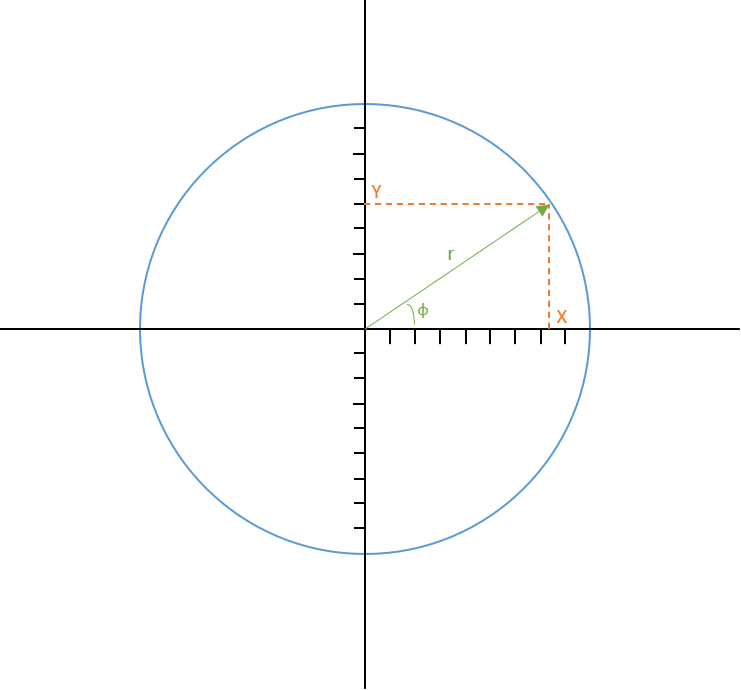
\includegraphics[width=10.29in]{./images/spacial/coor_pol_car} 

}

\caption{Polar and Cartesian Coordinates}\label{fig:polcar}
\end{figure}

Figure \ref{fig:polcar} shows

\section*{Exploratory Spacial Data Analysis (ESDA)}\label{exploratory-spacial-data-analysis-esda}
\addcontentsline{toc}{section}{Exploratory Spacial Data Analysis (ESDA)}

\begin{itemize}
\item
  It is another way to call spacial statistics methods.
\item
  \key{ESDA} is the starting point to prove if spacial correlation is present.
\item
  Conclusions from the ESDA, the hypothesis of spacial randomness can be rejected, to look for spacial conglomerates. It also helps with the spacial specification of the models.
\item
  There are two types of measurements:

  \begin{itemize}
  \item
    Global measurements: Indicator of spacial autocorrelation or general similarity between regions. Its disadvantage is to average.
  \item
    Local measurements: These statistics are determined for each region. There is no generalization of the area. Makes possible to compare between regions if they are similar or different.
  \end{itemize}
\end{itemize}

\subsection*{Spacial autocorrelation}\label{spacial-autocorrelation}
\addcontentsline{toc}{subsection}{Spacial autocorrelation}

\begin{itemize}
\item
  \defi{Spacial autocorrelation}: Happens when variables are correlated with the location. It means that observations that are closer have more similarities in between than the distant ones. That means that knowing the values of a location can help predicting the near ones.
\item
  The \key{degree of autocorrelation} is another concept that can be looked for. It is the distance from where the observations become independent.
\item
  \key{Global autocorrelation} can be measured using \key{Moran's I statistics} and \key{Geary's C}.
\item
  The most popular local measurements are part of the \key{Local Indicator of Spacial Association (LISA)}. It includes \key{Moran's $I_i$ statistics} and \key{Geary's $C_i$ local statistics}.
\item
  Global statistics can identify conglomerates and spacial relationships just for all the system, but they can be disaggregated into local statistics to detect local spacial relationship paterns between regions.
\end{itemize}

\subsubsection*{Moran's I}\label{morans-i}
\addcontentsline{toc}{subsubsection}{Moran's I}

\begin{itemize}
\item
  \(H_0\): No spacial autocorrelation; i.e.~the values are randomly distributed.
\item
  \(I>0\): Positive spacial autocorrelation. The values to the distance are similar.
\item
  \(I<0\): Negative spacial autocorrelation. The values to the distance are different.
\item
  \(I=0\): The values to the distance are randomly distributed.
\end{itemize}

\begin{Shaded}
\begin{Highlighting}[]
\FunctionTok{moran}\NormalTok{()}
\FunctionTok{moran.test}\NormalTok{()}
\FunctionTok{moran.mc}\NormalTok{()}
\FunctionTok{moran.plot}\NormalTok{()}
\end{Highlighting}
\end{Shaded}

\subsubsection*{Geary's C}\label{gearys-c}
\addcontentsline{toc}{subsubsection}{Geary's C}

\begin{itemize}
\item
  \(H_0\): No spacial autocorrelation; i.e.~the values are randomly distributed.
\item
  \(0<C>1\): Positive spacial autocorrelation. The values to the distance are similar.
\item
  \(1<C<2\): Negative spacial autocorrelation. The values to the distance are different.
\end{itemize}

\begin{Shaded}
\begin{Highlighting}[]
\FunctionTok{geary}\NormalTok{()}
\FunctionTok{geary.test}\NormalTok{()}
\FunctionTok{geary.mc}\NormalTok{()}
\end{Highlighting}
\end{Shaded}

\subsection*{Assumptions}\label{assumptions}
\addcontentsline{toc}{subsection}{Assumptions}

\begin{itemize}
\item
  \key{Estationarity}. The analized data must be normal distributed with constant mean and variance.

  \begin{itemize}
  \tightlist
  \item
  \end{itemize}
\end{itemize}

\chapter{Parts}\label{parts}

You can add parts to organize one or more book chapters together. Parts can be inserted at the top of an .Rmd file, before the first-level chapter heading in that same file.

Add a numbered part: \texttt{\#\ (PART)\ Act\ one\ \{-\}} (followed by \texttt{\#\ A\ chapter})

Add an unnumbered part: \texttt{\#\ (PART\textbackslash{}*)\ Act\ one\ \{-\}} (followed by \texttt{\#\ A\ chapter})

Add an appendix as a special kind of un-numbered part: \texttt{\#\ (APPENDIX)\ Other\ stuff\ \{-\}} (followed by \texttt{\#\ A\ chapter}). Chapters in an appendix are prepended with letters instead of numbers.

\chapter{Footnotes and citations}\label{footnotes-and-citations}

\section{Footnotes}\label{footnotes}

Footnotes are put inside the square brackets after a caret \texttt{\^{}{[}{]}}. Like this one \footnote{This is a footnote.}.

\section{Citations}\label{citations}

Reference items in your bibliography file(s) using \texttt{@key}.

For example, we are using the \textbf{bookdown} package \citep{R-bookdown} (check out the last code chunk in index.Rmd to see how this citation key was added) in this sample book, which was built on top of R Markdown and \textbf{knitr} \citep{xie2015} (this citation was added manually in an external file book.bib).
Note that the \texttt{.bib} files need to be listed in the index.Rmd with the YAML \texttt{bibliography} key.

The RStudio Visual Markdown Editor can also make it easier to insert citations: \url{https://rstudio.github.io/visual-markdown-editing/\#/citations}

\chapter{Blocks}\label{blocks}

\section{Equations}\label{equations}

Here is an equation.

\begin{equation} 
  f\left(k\right) = \binom{n}{k} p^k\left(1-p\right)^{n-k}
  \label{eq:binom}
\end{equation}

You may refer to using \texttt{\textbackslash{}@ref(eq:binom)}, like see Equation \eqref{eq:binom}.

\section{Theorems and proofs}\label{theorems-and-proofs}

Labeled theorems can be referenced in text using \texttt{\textbackslash{}@ref(thm:tri)}, for example, check out this smart theorem \ref{thm:tri}.

\begin{theorem}
\protect\hypertarget{thm:tri}{}\label{thm:tri}For a right triangle, if \(c\) denotes the \emph{length} of the hypotenuse
and \(a\) and \(b\) denote the lengths of the \textbf{other} two sides, we have
\[a^2 + b^2 = c^2\]
\end{theorem}

Read more here \url{https://bookdown.org/yihui/bookdown/markdown-extensions-by-bookdown.html}.

\section{Callout blocks}\label{callout-blocks}

The R Markdown Cookbook provides more help on how to use custom blocks to design your own callouts: \url{https://bookdown.org/yihui/rmarkdown-cookbook/custom-blocks.html}

\chapter{Sharing your book}\label{sharing-your-book}

\section{Publishing}\label{publishing}

HTML books can be published online, see: \url{https://bookdown.org/yihui/bookdown/publishing.html}

\section{404 pages}\label{pages}

By default, users will be directed to a 404 page if they try to access a webpage that cannot be found. If you'd like to customize your 404 page instead of using the default, you may add either a \texttt{\_404.Rmd} or \texttt{\_404.md} file to your project root and use code and/or Markdown syntax.

\section{Metadata for sharing}\label{metadata-for-sharing}

Bookdown HTML books will provide HTML metadata for social sharing on platforms like Twitter, Facebook, and LinkedIn, using information you provide in the \texttt{index.Rmd} YAML. To setup, set the \texttt{url} for your book and the path to your \texttt{cover-image} file. Your book's \texttt{title} and \texttt{description} are also used.

This \texttt{gitbook} uses the same social sharing data across all chapters in your book- all links shared will look the same.

Specify your book's source repository on GitHub using the \texttt{edit} key under the configuration options in the \texttt{\_output.yml} file, which allows users to suggest an edit by linking to a chapter's source file.

Read more about the features of this output format here:

\url{https://pkgs.rstudio.com/bookdown/reference/gitbook.html}

Or use:

\begin{Shaded}
\begin{Highlighting}[]
\NormalTok{?bookdown}\SpecialCharTok{::}\NormalTok{gitbook}
\end{Highlighting}
\end{Shaded}


  \bibliography{book.bib,packages.bib}

\end{document}
